% 26-11.tex -- Integrali tripli (formule di riduzione, coordinate sferiche)
%             e Superfici regolari (26/11/2026)
\section{Integrali tripli}

\pencilnote{Prima della definizione di integrale triplo, occorre la definizione di dominio normale in $\mathbb{R}^3$.}

\begin{definition}[Dominio normale rispetto al piano $(x, y)$]
Un insieme $E \subseteq \mathbb{R}^3$ si dice \underline{normale rispetto al piano $(x, y)$} se
\[
E = \{ (x, y, z) \in \mathbb{R}^3 : (x, y) \in D \text{ dominio normale di } \mathbb{R}^2 \text{ e } \alpha(x, y) \le z \le \beta(x, y) \}
\]
con $\alpha, \beta : D \to \mathbb{R}$ continue e $\alpha(x, y) \le \beta(x, y)$ per ogni $(x, y) \in D$.

\begin{center}
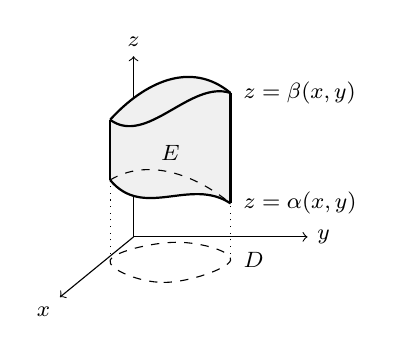
\begin{tikzpicture}[scale=0.85]
    \draw[->] (0,0) -- (2.6,0) node[right] {\footnotesize $y$};
    \draw[->] (0,0) -- (0,2.7) node[above] {\footnotesize $z$};
    \draw[->] (0,0) -- (-1.1,-0.9) node[below left] {\footnotesize $x$};

    % Proiezione D sul piano xy (dominio generico)
    \draw[dashed] plot[smooth cycle, tension=0.75] coordinates {
        (-0.35,-0.35) (0.45,-0.68) (1.45,-0.35) (0.65,-0.08)
    };
    \node[right] at (1.5,-0.35) {\footnotesize $D$};

    % Linee di proiezione verticale
    \draw[dotted] (-0.35,-0.35) -- (-0.35,0.85);
    \draw[dotted] (1.45,-0.35) -- (1.45,0.50);

    % Riempimento leggero del cilindroide E
    \fill[gray!12] (-0.35,0.85)
        .. controls (0.15,0.25) and (0.85,0.90) .. (1.45,0.50)
        -- (1.45,2.15)
        .. controls (0.85,2.65) and (0.15,2.30) .. (-0.35,1.75)
        -- cycle;

    % Superficie inferiore z = alpha(x, y) (inclinata e ondulata)
    \draw[thick] (-0.35,0.85) .. controls (0.15,0.25) and (0.85,0.90) .. (1.45,0.50);
    \draw[dashed] (-0.35,0.85) .. controls (0.20,1.18) and (0.90,0.95) .. (1.45,0.50);

    % Superficie superiore z = beta(x, y) (inclinata in senso opposto e ondulata)
    \draw[thick] (-0.35,1.75) .. controls (0.20,1.35) and (0.85,2.35) .. (1.45,2.15);
    \draw[thick] (-0.35,1.75) .. controls (0.15,2.30) and (0.85,2.65) .. (1.45,2.15);

    % Generatrici verticali laterali
    \draw[thick] (-0.35,0.85) -- (-0.35,1.75);
    \draw[thick] (1.45,0.50) -- (1.45,2.15);

    % Etichette
    \node at (0.55,1.25) {\footnotesize $E$};
    \node[right] at (1.5,2.15) {\footnotesize $z = \beta(x, y)$};
    \node[right] at (1.5,0.50) {\footnotesize $z = \alpha(x, y)$};
\end{tikzpicture}
\end{center}

Per definizione, il volume (misura) di $E$ è:
\[
m(E) = \iint_D \big[ \beta(x, y) - \alpha(x, y) \big]\, dx\, dy
\]
\end{definition}

\begin{definition}[Partizione in domini normali]
Sia $E \subseteq \mathbb{R}^3$ un dominio normale. La famiglia $\mathcal{P} = \{ E_1, E_2, \dots, E_n \}$ si dice \underline{partizione di $E$ in domini normali} se:
\begin{enumerate}
    \item $E_i \subseteq \mathbb{R}^3$ è normale $\forall i = 1, \dots, n$;
    \item $\mathring{E}_i \cap \mathring{E}_j = \emptyset \quad \forall i \neq j$;
    \item $\displaystyle\bigcup_{i=1}^n E_i = E$.
\end{enumerate}
\end{definition}


\subsection{Definizione di integrale triplo e formule di riduzione}

\begin{definition}[Integrale triplo]
Sia $f : E \subseteq \mathbb{R}^3 \to \mathbb{R}$ una funzione \underline{limitata}, con $E$ dominio normale. Sia $\mathcal{P} = \{ E_1, \dots, E_N \}$ una partizione di $E$ in domini normali, ossia tale che:
\begin{enumerate}
    \item $E_i$ sono normali $\forall i = 1, \dots, N$;
    \item $\displaystyle\bigcup_{i=1}^N E_i = E$;
    \item $\mathring{E}_i \cap \mathring{E}_j = \emptyset \quad \forall i \neq j$.
\end{enumerate}
Posti
\[
m_i = \inf_{E_i} f, \qquad M_i = \sup_{E_i} f
\]
definiamo le somme integrali inferiore e superiore relative a $f$ e a $\mathcal{P}$:
\[
s(\mathcal{P}, f) = \sum_{i=1}^N m_i \cdot m(E_i), \qquad S(\mathcal{P}, f) = \sum_{i=1}^N M_i \cdot m(E_i)
\]
Si dimostra che per ogni coppia di partizioni $\mathcal{P}, \mathcal{Q}$ risulta $s(\mathcal{P}, f) \le S(\mathcal{Q}, f)$, quindi gli insiemi
\[
A = \{ s(\mathcal{P}, f) : \mathcal{P} \text{ partizione} \}, \qquad B = \{ S(\mathcal{P}, f) : \mathcal{P} \text{ partizione} \}
\]
sono separati. Se $\inf B = \sup A = c$, allora $f$ si dice \underline{integrabile} in $E$ e l'elemento di separazione
\[
c = \iiint_E f(x, y, z)\, dx\, dy\, dz
\]
si chiama \underline{integrale triplo} di $f$ su $E$.
\end{definition}

\begin{theorem}[Formule di riduzione per gli integrali tripli]
Sia $f : E \subseteq \mathbb{R}^3 \to \mathbb{R}$ continua.

\begin{enumerate}
    \item \textbf{Formula di riduzione per fili:} se $E$ è normale rispetto al piano $(x, y)$, ovvero
    \[
    E = \{ (x, y, z) \in \mathbb{R}^3 : (x, y) \in D, \ \alpha(x, y) \le z \le \beta(x, y) \}
    \]
    allora
    \[
    \iiint_E f(x, y, z)\, dx\, dy\, dz = \iint_D \left[ \int_{\alpha(x, y)}^{\beta(x, y)} f(x, y, z)\, dz \right] dx\, dy
    \]

    \item \textbf{Formula di riduzione per strati:} detto $E_z = \{ (x, y) \in \mathbb{R}^2 : (x, y, z) \in E \}$ la sezione orizzontale di $E$ a quota $z \in [z_{\min}, z_{\max}]$, si ha
    \[
    \iiint_E f(x, y, z)\, dx\, dy\, dz = \int_{z_{\min}}^{z_{\max}} \left[ \iint_{E_z} f(x, y, z)\, dx\, dy \right] dz
    \]
\end{enumerate}

\begin{center}
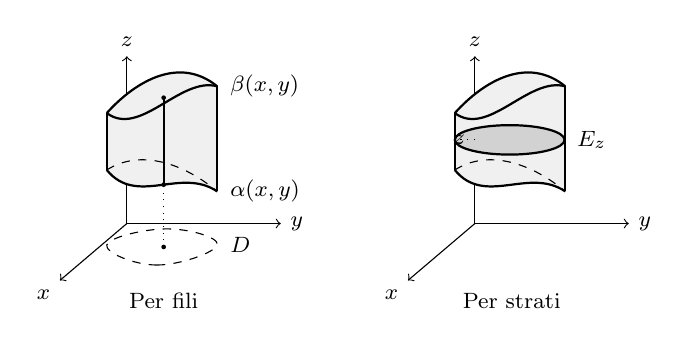
\begin{tikzpicture}[scale=0.85]
    % Schema 1: Riduzione per fili
    \begin{scope}[shift={(-2.6,0)}]
        \draw[->] (0,0) -- (2.3,0) node[right] {\footnotesize $y$};
        \draw[->] (0,0) -- (0,2.5) node[above] {\footnotesize $z$};
        \draw[->] (0,0) -- (-1.0,-0.85) node[below left] {\footnotesize $x$};

        % Proiezione D
        \draw[dashed] plot[smooth cycle, tension=0.75] coordinates {
            (-0.3,-0.32) (0.45,-0.62) (1.35,-0.32) (0.6,-0.08)
        };
        \node[right] at (1.4,-0.32) {\footnotesize $D$};

        % Cilindroide E
        \fill[gray!12] (-0.3,0.8)
            .. controls (0.15,0.25) and (0.8,0.85) .. (1.35,0.48)
            -- (1.35,2.05)
            .. controls (0.8,2.5) and (0.15,2.15) .. (-0.3,1.65)
            -- cycle;
        \draw[thick] (-0.3,0.8) .. controls (0.15,0.25) and (0.8,0.85) .. (1.35,0.48);
        \draw[dashed] (-0.3,0.8) .. controls (0.2,1.12) and (0.85,0.9) .. (1.35,0.48);
        \draw[thick] (-0.3,1.65) .. controls (0.2,1.28) and (0.8,2.2) .. (1.35,2.05);
        \draw[thick] (-0.3,1.65) .. controls (0.15,2.15) and (0.8,2.5) .. (1.35,2.05);
        \draw[thick] (-0.3,0.8) -- (-0.3,1.65);
        \draw[thick] (1.35,0.48) -- (1.35,2.05);

        % Filo verticale
        \draw[thick] (0.55,0.58) -- (0.55,1.88);
        \draw[dotted] (0.55,-0.35) -- (0.55,0.58);
        \fill (0.55,-0.35) circle (1pt);
        \fill (0.55,0.58) circle (1pt);
        \fill (0.55,1.88) circle (1pt);

        \node[right] at (1.4,2.05) {\footnotesize $\beta(x, y)$};
        \node[right] at (1.4,0.48) {\footnotesize $\alpha(x, y)$};
        \node[below] at (0.55,-0.9) {\footnotesize Per fili};
    \end{scope}

    % Schema 2: Riduzione per strati
    \begin{scope}[shift={(2.6,0)}]
        \draw[->] (0,0) -- (2.3,0) node[right] {\footnotesize $y$};
        \draw[->] (0,0) -- (0,2.5) node[above] {\footnotesize $z$};
        \draw[->] (0,0) -- (-1.0,-0.85) node[below left] {\footnotesize $x$};

        % Cilindroide E
        \fill[gray!12] (-0.3,0.8)
            .. controls (0.15,0.25) and (0.8,0.85) .. (1.35,0.48)
            -- (1.35,2.05)
            .. controls (0.8,2.5) and (0.15,2.15) .. (-0.3,1.65)
            -- cycle;
        \draw[thick] (-0.3,0.8) .. controls (0.15,0.25) and (0.8,0.85) .. (1.35,0.48);
        \draw[dashed] (-0.3,0.8) .. controls (0.2,1.12) and (0.85,0.9) .. (1.35,0.48);
        \draw[thick] (-0.3,1.65) .. controls (0.2,1.28) and (0.8,2.2) .. (1.35,2.05);
        \draw[thick] (-0.3,1.65) .. controls (0.15,2.15) and (0.8,2.5) .. (1.35,2.05);
        \draw[thick] (-0.3,0.8) -- (-0.3,1.65);
        \draw[thick] (1.35,0.48) -- (1.35,2.05);

        % Strato orizzontale E_z
        \fill[gray!35] (0.52,1.25) ellipse (0.82 and 0.22);
        \draw[thick] (0.52,1.25) ellipse (0.82 and 0.22);
        \draw[dotted] (0,1.25) node[left] {\footnotesize $z$} -- (-0.3,1.25);
        \node[right] at (1.38,1.25) {\footnotesize $E_z$};
        \node[below] at (0.55,-0.9) {\footnotesize Per strati};
    \end{scope}
\end{tikzpicture}
\end{center}
\end{theorem}

\begin{esercizio}[EXE 1]
Calcolare
\[
\iiint_E z\, dx\, dy\, dz, \qquad E = \{ (x, y, z) \in \mathbb{R}^3 : x^2 + y^2 \le z \le 1, \ y \ge 0 \}
\]
La proiezione sul piano $(x, y)$ è il semicerchio $D = \{ x^2 + y^2 \le 1, \ y \ge 0 \}$.

\textbf{1) Per fili:}
\begin{align*}
\iiint_E z\, dx\, dy\, dz
&= \iint_D \left[ \int_{x^2 + y^2}^1 z\, dz \right] dx\, dy
= \iint_D \frac{1 - (x^2 + y^2)^2}{2}\, dx\, dy \\
&= \frac{1}{2} \int_0^\pi \left[ \int_0^1 \rho (1 - \rho^4)\, d\rho \right] d\theta
= \frac{\pi}{2} \left[ \frac{\rho^2}{2} - \frac{\rho^6}{6} \right]_0^1
= \frac{\pi}{6}
\end{align*}

\textbf{2) Per strati:} si ha $z_{\min} = 0$, $z_{\max} = 1$ e, fissato $z \in [0, 1]$, la sezione $E_z = \{ x^2 + y^2 \le z, \ y \ge 0 \}$ è un semicerchio di raggio $\sqrt{z}$, quindi $m(E_z) = \dfrac{\pi z}{2}$:
\[
\iiint_E z\, dx\, dy\, dz
= \int_0^1 z \left[ \iint_{E_z} dx\, dy \right] dz
= \int_0^1 z \left( \frac{\pi z}{2} \right) dz
= \frac{\pi}{6}
\]
\end{esercizio}

\begin{esercizio}[EXE 2]
Calcolare
\[
\iiint_E x y z\, dx\, dy\, dz, \qquad E = \{ (x, y, z) \in \mathbb{R}^3 : z^2 \le x^2 + y^2, \ z \ge x^2 + y^2 \}
\]
Poiché $z \ge x^2 + y^2 \ge 0$, la condizione $z^2 \le x^2 + y^2$ equivale a $z \le \sqrt{x^2 + y^2}$. Dunque:
\[
x^2 + y^2 \le z \le \sqrt{x^2 + y^2} \iff \sqrt{x^2 + y^2} \le 1 \implies D = \left\{ \sqrt{x^2 + y^2} \le 1 \right\}
\]
Integrando per fili e passando in coordinate polari:
\begin{align*}
\iiint_E x y z\, dx\, dy\, dz
&= \iint_D \left[ \int_{x^2 + y^2}^{\sqrt{x^2 + y^2}} x y z\, dz \right] dx\, dy
= \iint_D x y \left[ \frac{x^2 + y^2 - (x^2 + y^2)^2}{2} \right] dx\, dy \\
&= \frac{1}{2} \int_0^{2\pi} \left[ \int_0^1 \rho^3 \cos\theta \sin\theta (\rho^2 - \rho^4)\, d\rho \right] d\theta
= 0
\end{align*}
\end{esercizio}

\subsection{Coordinate sferiche}

\[
\begin{cases}
x = \rho \sin\theta \cos\varphi \\
y = \rho \sin\theta \sin\varphi \\
z = \rho \cos\theta
\end{cases}
\qquad \text{con } \rho \ge 0, \ \theta \in [0, \pi], \ \varphi \in [0, 2\pi]
\]
Lo \underline{Jacobiano} della trasformazione è:
\[
\left| \frac{\partial(x, y, z)}{\partial(\rho, \theta, \varphi)} \right| = \rho^2 \sin\theta
\]

\begin{center}
\begin{tikzpicture}[scale=1.0]
    \draw[->] (0,0) -- (2.8,0) node[right] {\footnotesize $y$};
    \draw[->] (0,0) -- (0,2.7) node[above] {\footnotesize $z$};
    \draw[->] (0,0) -- (-1.4,-1.1) node[below left] {\footnotesize $x$};

    \coordinate (O) at (0,0);
    \coordinate (P) at (1.2,1.9);
    \coordinate (Pxy) at (1.2,-0.55);

    % Raggio rho e proiezione sul piano xy
    \draw[thick] (O) -- (P) node[midway, left] {\footnotesize $\rho$};
    \draw[dashed] (O) -- (Pxy);
    \draw[dashed] (P) -- (Pxy);
    \fill (P) circle (1.4pt) node[above right] {\footnotesize $(x, y, z)$};
    \fill (Pxy) circle (1.2pt) node[below right] {\footnotesize $(x, y, 0)$};

    % Angolo theta (colatitudine dall'asse z)
    \draw[->] (0,0.65) arc (90:58:0.65);
    \node[above] at (0.22,0.62) {\footnotesize $\theta$};

    % Angolo phi (azimut dall'asse x)
    \draw[->] (-0.52,-0.41) arc (-142:-25:0.65);
    \node[below] at (-0.05,-0.55) {\footnotesize $\varphi$};
\end{tikzpicture}
\end{center}

